%% here. Need to make the problem description and solution to E.6 and F.6 look like B.6 and C.6

From HW~E.4, the linearized equations of motion are given by
\[
\begin{pmatrix}
m_1 & 0 \\ 0 & \left( \frac{m_2 \ell^2}{3} + m_1 z_e^2 \right)
\end{pmatrix} \begin{pmatrix}\ddot{\tilde{z}} \\ \ddot{\tilde{\theta}} \end{pmatrix}
= \begin{pmatrix} -m_1 g \tilde{\theta} \\ \ell \tilde{F} - m_1 g \tilde{z} \end{pmatrix}.
\]
%
These can be expressed as
\begin{align*}
	\ddot{\tilde{z}} + g\tilde{\theta} &= 0 \\
	\left( \frac{m_2 \ell^2}{3} + m_1 z_e^2 \right) \ddot{\tilde{\theta}}  + m_1 g\tilde{z} &= \ell \tilde{F}.
\end{align*}
%
To simplify the notation in the following discussion, define
\[
A \defeq \frac{m_2 \ell^2}{3} + m_1 z_e^2
\]
and substitute into the second equation of motion to give
\begin{align*}
	\ddot{\tilde{z}} + g\tilde{\theta} &= 0 \\
	A \ddot{\tilde{\theta}}  + m_1 g\tilde{z} &= \ell \tilde{F}.
\end{align*}
%
Taking the Laplace transform with initial conditions set to zero and rearranging gives
\begin{align}
	s^2 \tilde{Z}(s) + g \tilde{\Theta}(s) &=0 \label{eq:soln_E6_1}\\
	m_1 g \tilde{Z}(s) + A s^2\tilde{\Theta}(s) &= \ell\tilde{F}(s) .
\label{eq:soln_E6_2}
\end{align}

To form the transfer functions, we are interested in solving for $\tilde{Z}(s)$ and $\tilde{\Theta}(s)$ in terms of $\tilde{F}(s)$. To do this, write~\eqref{eq:soln_E6_1} and \eqref{eq:soln_E6_2} in matrix form as
\[
\left(\begin{array}{c|c}
s^2 & g \\\hline m_1g & As^2 \end{array}\right)
\begin{pmatrix}\tilde{Z}(s) \\ \tilde{\Theta}(s) \end{pmatrix} 
= \begin{pmatrix} 0 \\ \ell \end{pmatrix} \tilde{F}(s),
\]
and invert the matrix on the left hand side to obtain
\begin{align*}
     \frac{\tilde{Z}(s)}{\tilde{F}(s)} &= \frac{-g\ell}{As^4-m_1g^2} \\
     \frac{\tilde{\Theta}(s)}{\tilde{F}(s)} &= \frac{\ell s^2}{As^4-m_1g^2} .
\end{align*}
%
Directly from~\eqref{eq:soln_E6_1} we also find that 
\[
     \frac{\tilde{Z}(s)}{\tilde{\Theta}(s)} = -\frac{g}{s^2}. 
\]

If we neglect the effect of the gravity torque produced by motion of the ball away from the equilibrium position, then the $m_1 g \tilde{Z}(s)$ term in equation~\eqref{eq:soln_E6_2} drops out and the transfer function from force to angular position simplifies to 
\[
     \frac{\tilde{\Theta}(s)}{\tilde{F}(s)} = \frac{\ell}{As^2} .
\]
This assumption implies that the input force influences the beam angle and that the beam angle influences the ball position, but that the ball position does not influence the beam angle.
%
The block diagram for the simplified system is shown in Figure~\ref{fig:hw_ballbeam_block_diagram}
\begin{figure}[htbp]
   \centering
   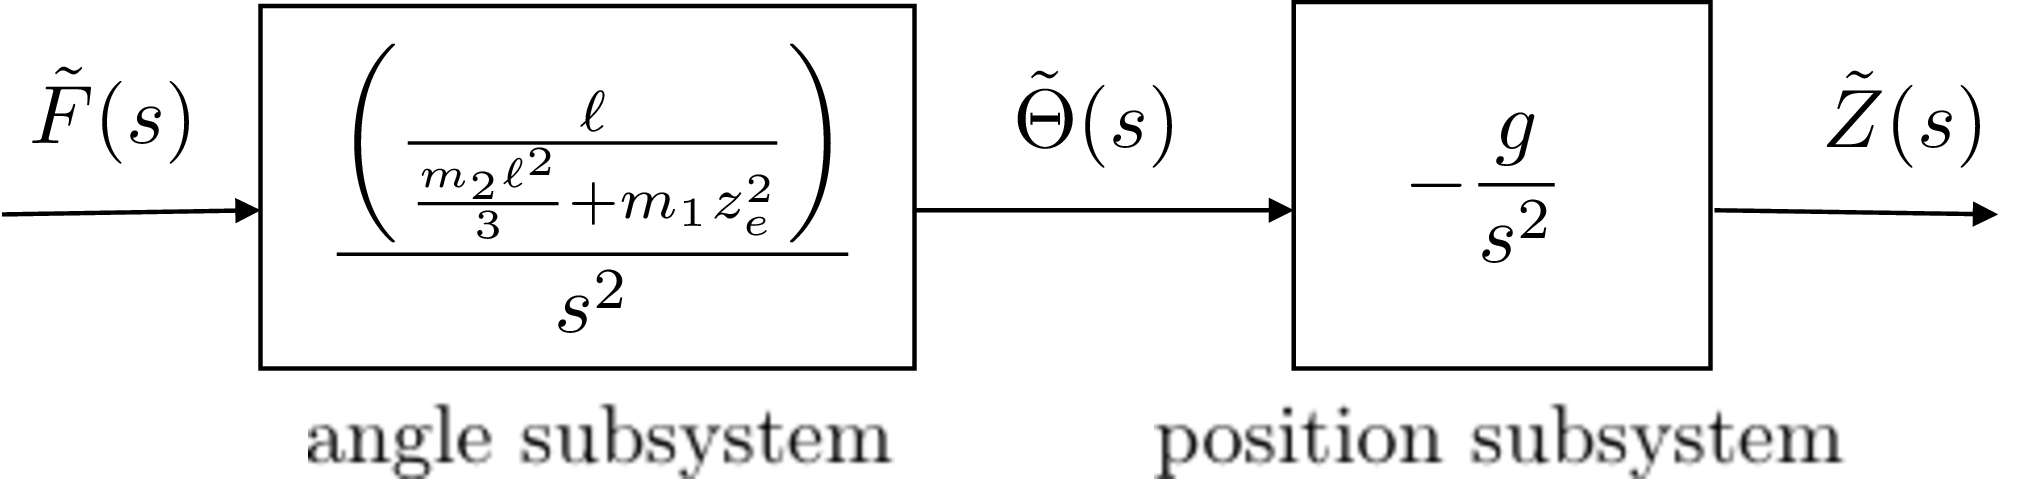
\includegraphics[width=0.8\textwidth]{6_design_studies/figures/hw_ballbeam_block_diagram.pdf}
   \caption{The ball-on-beam dynamics are approximated by cascade of two subsystem transfer functions.}
   \label{fig:hw_ballbeam_block_diagram} 
\end{figure}

The cascade approximation makes sense physically because the force on the beam directly affects the angle of the beam, which then influences the motion and position of the ball.
